%\chapter{De Vuelta a América. Cartagena de Indias}

Regresó a América con los navíos Fuerte y Conquistador en 1737 como
comandante general de Cartagena de Indias, plaza que tuvo que defender
de un sitio (1741) al que la había sometido el ataque del almirante
inglés Edward Vernon.\footnote{Artículo principal:
  \href{https://is.gd/m45nMc}{Sitio de Cartagena de Indias (1741)}} En
los primeros años en Cartagena, Lezo se encargó de labores de
guardacostas, que debían desbaratar el creciente contrabando, que
acabó precipitando la nueva guerra con el \index{Reino Unido} Reino
Unido. Con este mismo objetivo, creó junto con el gobernador de
Cartagena una compañía de armadores de corso. El contrabando británico
había crecido aprovechando las concesiones comerciales que el Reino
Unido había obtenido en el Tratado de Utrecht:\index{Tratado!de
  Utrecht} al comercio legal ---quinientas toneladas ampliadas a mil
en 1716, se unieron pronto los contrabandistas, que amenazaban el
comercio español y trataban de no pagar los derechos (impuestos) a la
Corona. A pesar de la renuencia del Gobierno británico a enfrentarse a
España y favorecer así su acercamiento a Francia, las quejas de los
comerciantes afectados por las actividades de los guardacostas y el
debilitamiento del gabinete de Horace Walpole acabaron por aumentar la
tensión entre los dos países y condujeron finalmente a la guerra.

\begin{figure}[!hbp]
\centering
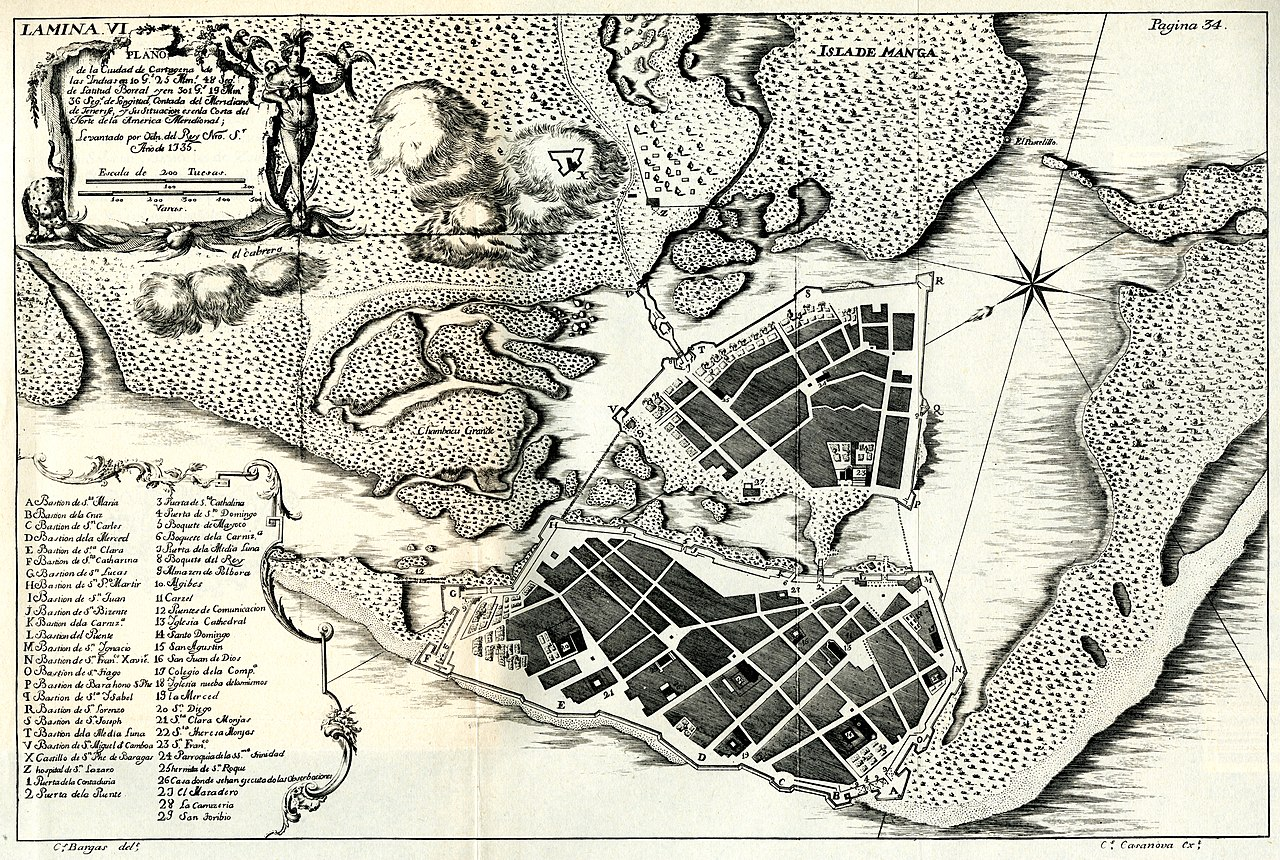
\includegraphics[width=.35\textwidth]{jpg_Plano_de_Cartagena_de_las_Indias_(1735).jpg}
\caption{\label{fig:planoCartagena} Plano de Cartagena de las Indias
  realizado en 1735 y publicado en la obra Relación histórica del
  viaje a la América meridional, de Jorge Juan y Antonio de Ulloa.}
\end{figure}

La justificación de los británicos para iniciar un conflicto con
España fue, entre otros muchos incidentes, el apresamiento de un barco
mercante mandado por Robert Jenkins \index{Jenkins} cerca de la costa
de Florida \index{Florida} en 1731. Juan de León Fandiño apresó el
barco y supuestamente cortó la oreja de su capitán al tiempo que le
decía: «Aquí está tu oreja: tómala y llévasela al rey de Inglaterra,
para que sepa que aquí no se contrabandea». A la sazón, el tráfico de
ultramar español se componía en gran parte del contrabando.

Rechazado en La Guaira el 22 de octubre de 1739, de la que había
pensado apoderarse sin encontrar resistencia, Vernon conquistó la
plaza de Portobelo (Panamá) en noviembre, y desafió a Lezo, a lo que
el marino español contestó:

\begin{displayquote}
{[\ldots]} puedo asegurar a V. E. que si me hubiera hallado en Portobelo
para impedírselo, y si las cosas hubieran ido a mi satisfacción, aun
para buscarle en cualquier otra parte, persuadiéndome que el ánimo que
faltó a los de Portobelo, me hubiera sobrado para contener su cobardía
[en referencia a los defensores del lugar, que la entregaron sin
resistencia].
\end{displayquote}

A continuación y de acuerdo al plan trazado, que los españoles
conocían por los informes de un espía que trabajaba en Jamaica, Vernon
\index{Vernon} se dirigió \index{Cartagena!de Indias|textbf} en
marzo de 1741 contra Cartagena. Antes había realizado dos ataques
exploratorios, con escasas fuerzas, en marzo y mayo de 1740, que Lezo
rechazó.

La flota británica sumaba dos mil cañones dispuestos en casi ciento
ochenta barcos, entre navíos de tres puentes (ocho), navíos de línea
(veintiocho), fragatas (doce), bombardas (dos) y buques de transporte
(ciento treinta), y en torno a treinta mil combatientes entre marinos
(quince mil), soldados (nueve mil regulares y cuatro mil de las
milicias norteamericanas) y esclavos negros macheteros de Jamaica
(cuatro mil).103 Las defensas de Cartagena incluían tres mil hombres
entre tropa regular (unos mil setecientos ochenta), milicianos
(quinientos), seiscientos indios flecheros traídos del interior, más
la cuantiosa marinería y tropa de desembarco de los seis navíos de
guerra de los que disponía la ciudad (ciento cincuenta hombres): el
Galicia, que era la nave capitana, el San Felipe, el San Carlos, el
África, el Dragón y el Conquistador. Tras tomar algunas de las
defensas de la ciudad, el asalto británico al castillo San Felipe de
Barajas, el último baluarte importante que la defendía, fracasó el 20
de abril; con gran parte de la tropa enferma, grandes bajas sufridas
en los combates y la llegada de la época de lluvias, los británicos
optaron por destruir las defensas a su alcance y abandonar el
asedio.

\begin{figure}[!hbp]
\centering
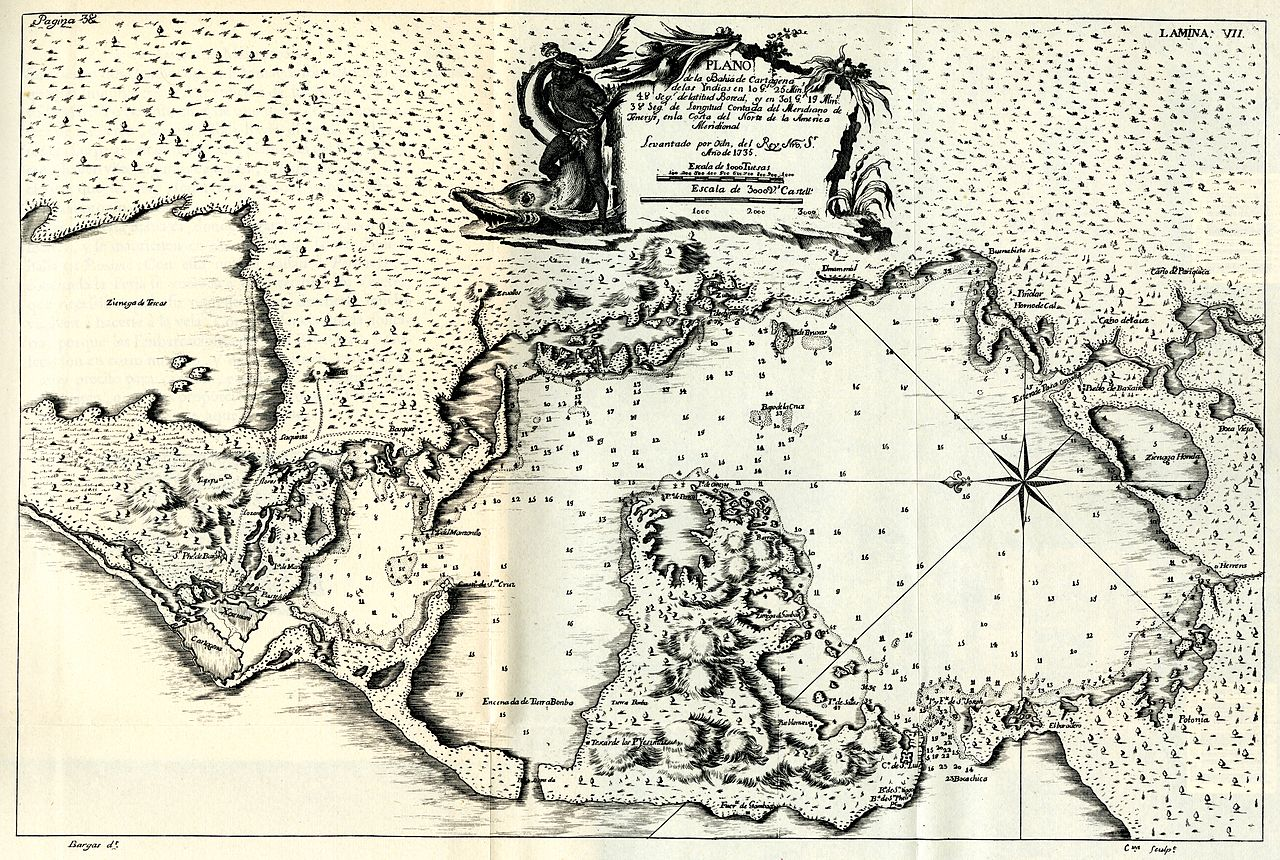
\includegraphics[width=.35\textwidth]{jpg_Plano_de_la_Bahia_de_Cartagena_de_las_Indias_(1735).jpg}
\caption{\label{fig:planoBahiaCartagena} Plano de la Bahía de
  Cartagena de Indias realizado en 1735 y publicado en la Obra
  Relación histórica del viaje a la América meridional, de Jorge Juan
  y Antonio de Ulloa.}
\end{figure}

\index{Cartagena!de Indias}
Las pérdidas británicas fueron graves: unos cuatro mil quinientos
muertos, seis barcos perdidos y entre diecisiete y veinte muy
dañados. Estas últimas obligaron al Gobierno británico a concentrar
sus fuerzas en las defensa de la metrópoli, el Atlántico septentrional
y el Mediterráneo, y a desechar nuevas campañas en las colonias
españolas en América. La derrota en Cartagena desbarató los planes
británicos para la campaña y permitió que continuase el dominio
español en la región durante varias décadas más. Los ingleses, que
contaban con la victoria, se habían precipitado a acuñar monedas y
medallas para celebrarla.108 Dichas medallas decían en su anverso:
«Los héroes británicos tomaron Cartagena el 1 de abril de 1741» y «El
orgullo español humillado por Vernon».
